\section{Entwurfsmuster}

\textbf{Entwurfsmuster} (\textit{Design Patterns}) sind wie Analyse- (s. Abschnitt~\ref{sec:analysemuster}) und Architekturmuster (s. Abschnitt~\ref{sec:architekturmuster}) vorgefertigte Lösungsschablonen für verallgemeinerte Probleme des Entwurfs.\\

\noindent
Entwurfsmuster müssen zur Lösung konkreter Aufgaben angepaßt werden.

\subsection{Beobachter (Observer)}

\subsubsection*{Problem}
\begin{itemize}
    \item eine Klasse soll die Möglichkeit haben, anderen Klassen Nachrichten zu senden
    \item der Typ der empfangenden Klasse soll vorher nicht bekannt sein
\end{itemize}

\subsubsection*{Lösung}
\begin{itemize}
    \item eine Klasse, die vom Typ \code{Observable} ist, besitzt Referenzen auf Objekte, die \code{Observer} (\textit{Nachrichtenempfänger})implementieren
    \item Beobachter registrieren sich bei den zu beobachtenden Objekten
    \item Nachrichten werden ausgehend von \code{Observable} (bspw. über \code{notify()}) an die \code{Observer} geschickt
\end{itemize}

Das Entwurfsmuster ist auch unter \textit{publish-subscribe} bekannt.


\begin{figure}
    \centering
    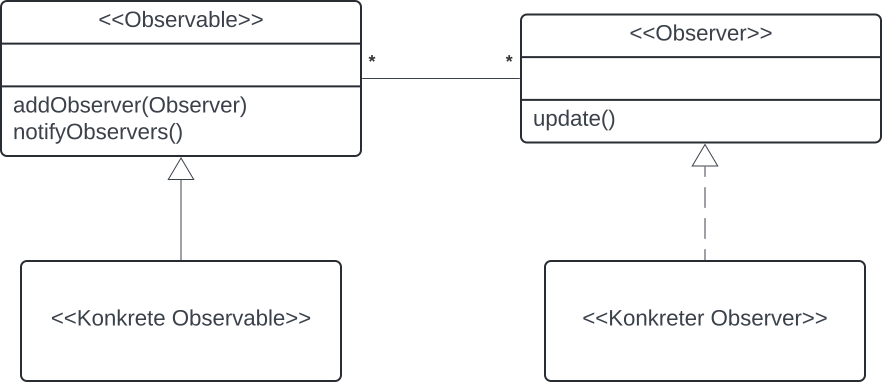
\includegraphics[scale=0.4]{part two/Objektorientierter Entwurf/img/observer}
    \caption{Klassendiagramm des Observer-Patterns (Quelle: eigene)}
    \label{fig:observer}
\end{figure}

\subsection{MVC (Model-View-Controller)}

\subsubsection*{Problem}

\begin{itemize}
    \item eine Anwendung verarbeitet Eingaben und reagiert (interaktiv) mit Ausgaben
    \item die Ausgaben sollen über eine Aktualisierung des GUI erfolgen
    \item es stellt sich die Frage, wie die Verantwortlichkeiten sinnvoll verteilt werden können
\end{itemize}

\subsubsection*{Lösung}
Die Verantwortlichkeiten werden unterteilt in

\begin{itemize}
    \item \textbf{Model} beinhalten Daten und fachliche Funktionalitäten
    \item \textbf{View} zeigen Daten (des Models) an
    \item \textbf{Controller} nehmen Eingabedaten entgegen, speichern Daten im Model und steuern Elemente des UI
\end{itemize}

\noindent
Hierbei reagiert die \textbf{View} auf Änderungen im \textbf{Model}, die View ist also ein \textbf{Beobachter} des Models (\textbf{Observable}).\\
Der \textbf{Controller} verarbeitet Nutzerinteraktionen und kommuniziert diese an das Model.\\
In der Hinsicht ist der Controller ein Observer für die GUI-Elemente, die Nutzerinteraktionen verarbeiten (s. Abbildung~\ref{fig:mvc}).

\begin{figure}
    \centering
    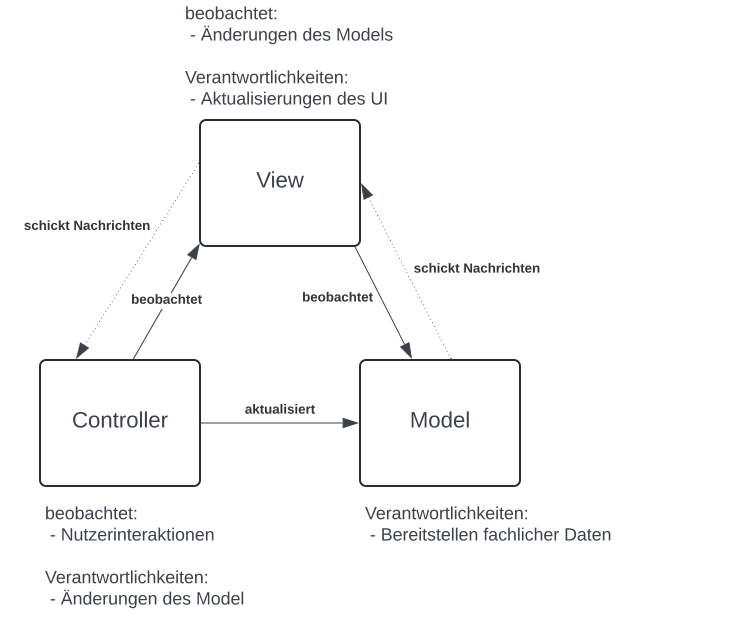
\includegraphics[scale=0.4]{part two/Objektorientierter Entwurf/img/mvc}
    \caption{Schematische Darstellung des MVC-Patterns mit seinen Verantwortlichkeiten (Quelle: eigene)}
    \label{fig:mvc}
\end{figure}

\subsubsection*{Vorteile}
Die Vorteile sind eine klare Trennung der Verantwortlichkeiten sowie die hierdurch bedingte lose Kopplung der Komponenten untereinander, was ein Testen sowie Austauschen der eingesetzten Komponenten vereinfacht.

\subsection{Immutable}\label{subsec:immutable}

\subsubsection*{Problem}
\begin{itemize}
    \item Referenzen auf Instanzen werden von einem Objekt an ein andere weitergegeben
    \item Änderungen der Inhalte der Referenzen wirken sich unerwünscht auf andere Objekte aus\footnote{
    auch bekannt als \textbf{Aliasing Bug}, s. \url{https://martinfowler.com/bliki/AliasingBug.html}, abgerufen 17.04.2024
    }
\end{itemize}

\subsubsection*{Beispiel}

\begin{minted}[mathescape,
    linenos,
    numbersep=5pt,
    gobble=2,
    fontsize=\small,
    frame=lines,
    framesep=2mm]{java}

    class Date {
        public Date(String d) {
            day = d;
        }
        public void setDay(String d) {
            day = d;
        }
    }

    class CalendarEvent {
        Date when;
        public CalendarEvent(Date w) {
            when = w;
        }
        public Date when() {
            return when;
        }
    }

    Date when = "Monday";
    CalendarEvent concertEvent = new CalendarEvent(when);
    CalendarEvent readingEvent = new CalendarEvent(when);

    // ändert gleichzeitig den Veranstaltungstag
    // von readingEvent
    concertEvent.getWhen().setDay("Tuesday");

\end{minted}


\subsubsection*{Lösung}

\begin{itemize}
    \item Attribute im Konstruktor definieren
    \item nur \code{get*}-Methoden implementieren, aber keine \code{set*}-Methoden
    \item es wird keine Methode implementiert, die den \textbf{internen Zustand} des Objektes verändert
    \item sollte eine Änderung des internen ZUstands benötigt sein, wird eine neue Instanz der Klasse mit den
    gewünschten Aktualisierungen erzeugt - das ursprüngliche Objekt bleibt so unverändert\footnote{
        Anwendung bspw. in \textbf{Value Object}s, vgl.~\cite[486]{Fow03}
    }
    \item die entsprechende Klasse sollte als \code{final} deklariert werden, damit es nicht möglich ist, abgeleitete Klassen zu erzeugen, in denen das Verhalten geändert wird
\end{itemize}

\subsubsection*{Probleme und Alternativen}
Sollten trotzdem die Eigenschaften eines Objektes oft geändert werden müssen, sollten die Klassen als \textit{mutable} implementiert werden, aber die \textit{Getter} der privaten Objekte sollten dann Kopien dieser Objekte zurückliefern.

\subsection{Iterator}

\subsubsection*{Problem}
\begin{itemize}
    \item Objekte sind in verschiedenen Datenstrukturen wie \textit{verkettete Liste}, \textit{Baum} oder \textit{Vektor} (sog. \textbf{Aggregaten}) organisiert
    \item sollen Methoden sequentiell auf alle Objekte zugreifen, die ein Aggregat beinhalten, muss für jede Datenstruktur der Zugriff anders organisiert werden\footnote{
    Baum wird in bestimmter Reihenfolge traversiert, auf ein Array wird über einen Laufindex zugegriffen usw.
    }
    \item dieStruktur soll verborgen bleiben, dam sie für den sequentiellen Zugriff unerheblich ist; die Datenstruktur wird darüber leicht austauschbar
\end{itemize}

\subsubsection*{Lösung}
Es wird von dem verwendeten Framework / der Programmiersprache ein \textbf{Iterator} zur Verfügung gestellt (s. Abbildung~\ref{fig:iterator}).


\begin{figure}
    \centering
    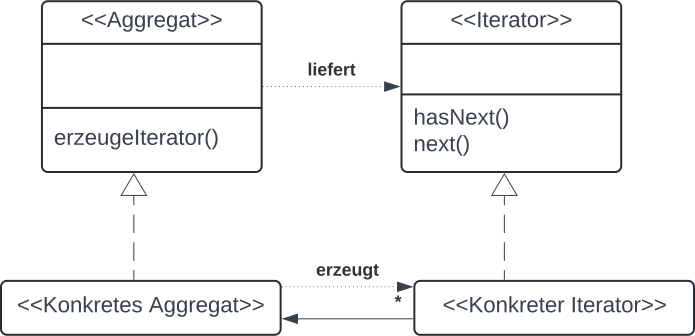
\includegraphics[scale=0.4]{part two/Objektorientierter Entwurf/img/iterator}
    \caption{Klassendiagramm des Iterator-Patterns (Quelle: in Anlehnung an~\cite[60, Abb. 3.9]{Wed09b})}
    \label{fig:iterator}
\end{figure}


\subsection{Fassade}

\subsubsection*{Problem}
\begin{itemize}
    \item Klassen nutzen eine zusammengehörige Gruppe von zusammenarbeitenden Klassen
    \item die Details der Gruppe sollen verborgen bleiben, damit einzelne BEstandteile leichter geändert oder ausgetauscht werden können
\end{itemize}

\subsubsection*{Lösung}
\begin{itemize}
    \item Bereitstellen einer Klasse, die eine \textbf{Fassade} repräsentiert
    \item die Klasse stellt Methoden bereits, die eine Untermenge der Funktionalität des Systems bereitstellt
    \item andere Klassen kennen die öffentliche Schnittstelle der Fassade und greifen nur noch auf diese zu
    \item die Fassade delegiert die Aufrufe an die Objekte, aus denen die Fassade besteht
\end{itemize}

\subsubsection*{Vorteile}
Die Fassade stellt die \textbf{Abstraktion der Gruppe} dar (vgl. \cite[61]{Wed09b}, s. Abbildung~\ref{fig:fassade}).

\begin{itemize}
    \item Benutzung der Gruppe von Klassen wird über einheitliche Schnittstelle vereinfacht
    \item Veränderungen hinter der Fassade bleiben ohne Auswirkungen auf die Nutzer der Fassade
    \item es ist nur die Schnittstelle der Fassade zu verstehen, nicht die Details der Gruppe
\end{itemize}

\begin{figure}
    \centering
    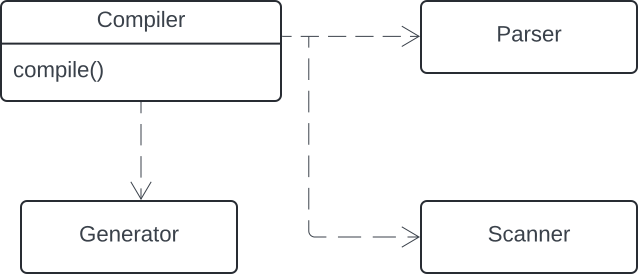
\includegraphics[scale=0.4]{part two/Objektorientierter Entwurf/img/fassade}
    \caption{Informelle Darstellung der Arbeitsweise einer Fassdade (Quelle: eigene)}
    \label{fig:fassade}
\end{figure}
